\documentclass{standalone}

% convert_magick -density 300 difference_symetrique.pdf difference_symetrique.png

\usepackage{tikz}
\usetikzlibrary{calc}

\begin{document}

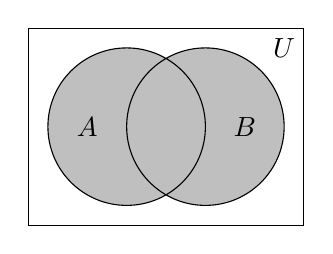
\begin{tikzpicture}
\draw (-1.25,-1.25) rectangle (2.25,1.25);
\draw[black, fill=lightgray] (0,0) circle (1) (1,0) circle (1);
\node at (-0.5,0) {$A$};
\node at (1.5,0) {$B$};
\node at (2,1) {$U$};
\end{tikzpicture}

\end{document}